


\tikzset{every picture/.style={line width=0.75pt}} %set default line width to 0.75pt        

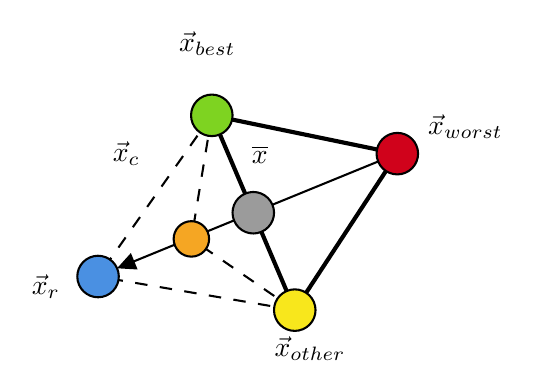
\begin{tikzpicture}[x=0.75pt,y=0.75pt,yscale=-1,xscale=1]
%uncomment if require: \path (0,914); %set diagram left start at 0, and has height of 914

%Straight Lines [id:da20472677135319306] 
\draw [line width=1.5]    (432.21,511.73) -- (521.59,530.19) ;
%Straight Lines [id:da15196510915112627] 
\draw [line width=1.5]    (472.18,605.58) -- (432.21,511.73) ;
%Straight Lines [id:da8014030305919331] 
\draw [line width=1.5]    (472.18,605.58) -- (521.59,530.19) ;
%Straight Lines [id:da3522320622069264] 
\draw    (521.59,530.19) -- (389.35,584.27) ;
\draw [shift={(386.58,585.41)}, rotate = 337.75] [fill={rgb, 255:red, 0; green, 0; blue, 0 }  ][line width=0.08]  [draw opacity=0] (8.93,-4.29) -- (0,0) -- (8.93,4.29) -- cycle    ;
%Shape: Circle [id:dp036939575554771675] 
\draw  [fill={rgb, 255:red, 155; green, 155; blue, 155 }  ,fill opacity=1 ] (442.99,562.57) .. controls (440.83,557.49) and (443.2,551.62) .. (448.28,549.45) .. controls (453.36,547.29) and (459.23,549.65) .. (461.4,554.74) .. controls (463.56,559.82) and (461.19,565.69) .. (456.11,567.85) .. controls (451.03,570.02) and (445.16,567.65) .. (442.99,562.57) -- cycle ;
%Shape: Circle [id:dp010246195714737727] 
\draw  [fill={rgb, 255:red, 208; green, 2; blue, 27 }  ,fill opacity=1 ] (512.39,534.1) .. controls (510.22,529.02) and (512.59,523.15) .. (517.67,520.99) .. controls (522.75,518.82) and (528.62,521.19) .. (530.79,526.27) .. controls (532.95,531.35) and (530.59,537.22) .. (525.51,539.39) .. controls (520.43,541.55) and (514.55,539.19) .. (512.39,534.1) -- cycle ;
%Straight Lines [id:da017687923938115357] 
\draw  [dash pattern={on 4.5pt off 4.5pt}]  (472.18,605.58) -- (377.4,589.39) ;
%Straight Lines [id:da40232054931076844] 
\draw  [dash pattern={on 4.5pt off 4.5pt}]  (432.21,511.73) -- (377.4,589.39) ;
%Shape: Circle [id:dp9492518387184166] 
\draw  [fill={rgb, 255:red, 74; green, 144; blue, 226 }  ,fill opacity=1 ] (386.58,585.41) .. controls (388.77,590.47) and (386.45,596.36) .. (381.38,598.56) .. controls (376.32,600.76) and (370.43,598.43) .. (368.23,593.37) .. controls (366.03,588.3) and (368.36,582.41) .. (373.42,580.21) .. controls (378.49,578.01) and (384.38,580.34) .. (386.58,585.41) -- cycle ;
%Straight Lines [id:da36492452425530564] 
\draw  [dash pattern={on 4.5pt off 4.5pt}]  (472.18,605.58) -- (422.36,571.27) ;
%Straight Lines [id:da2809967890037388] 
\draw  [dash pattern={on 4.5pt off 4.5pt}]  (432.21,511.73) -- (422.36,571.27) ;
%Shape: Circle [id:dp6259185945253334] 
\draw  [fill={rgb, 255:red, 126; green, 211; blue, 33 }  ,fill opacity=1 ] (423.01,515.65) .. controls (420.85,510.57) and (423.21,504.7) .. (428.29,502.53) .. controls (433.37,500.37) and (439.25,502.73) .. (441.41,507.81) .. controls (443.57,512.9) and (441.21,518.77) .. (436.13,520.93) .. controls (431.05,523.1) and (425.17,520.73) .. (423.01,515.65) -- cycle ;
%Shape: Circle [id:dp54940765139848] 
\draw  [fill={rgb, 255:red, 248; green, 231; blue, 28 }  ,fill opacity=1 ] (462.98,609.49) .. controls (460.82,604.41) and (463.18,598.54) .. (468.26,596.38) .. controls (473.34,594.21) and (479.22,596.58) .. (481.38,601.66) .. controls (483.54,606.74) and (481.18,612.61) .. (476.1,614.78) .. controls (471.02,616.94) and (465.14,614.58) .. (462.98,609.49) -- cycle ;
%Shape: Circle [id:dp024904628738977364] 
\draw  [fill={rgb, 255:red, 245; green, 166; blue, 35 }  ,fill opacity=1 ] (414.51,574.61) .. controls (412.66,570.28) and (414.68,565.26) .. (419.02,563.41) .. controls (423.35,561.56) and (428.37,563.58) .. (430.22,567.92) .. controls (432.06,572.26) and (430.05,577.28) .. (425.71,579.12) .. controls (421.37,580.97) and (416.35,578.95) .. (414.51,574.61) -- cycle ;

% Text Node
\draw (415,470) node [anchor=north west][inner sep=0.75pt]   [align=left] {$\displaystyle \vec{x}_{best}$};
% Text Node
\draw (535,510) node [anchor=north west][inner sep=0.75pt]   [align=left] {$\displaystyle \vec{x}_{worst}$};
% Text Node
\draw (461,617) node [anchor=north west][inner sep=0.75pt]   [align=left] {$\displaystyle \vec{x}_{other}$};
% Text Node
\draw (450,525) node [anchor=north west][inner sep=0.75pt]   [align=left] {$\displaystyle \overline{x}$};
% Text Node
\draw (344,587) node [anchor=north west][inner sep=0.75pt]   [align=left] {$\displaystyle \vec{x}_{r}$};
% Text Node
\draw (383,523) node [anchor=north west][inner sep=0.75pt]   [align=left] {$\displaystyle \vec{x}_{c}$};


\end{tikzpicture}